\section{Galaxy clustering and the effect of the photo-z quality cuts}
\label{sec:clustering}

We will now compute the angular galaxy correlations in the four photo-z bins of Fig.~\ref{Nz_bins}, before and after applying the different photo-z quality cuts of Fig.~\ref{sigvseff}. We want to see and characterize the impact of these cuts on clustering.

For this purpose, we use the Hierarchical Equal Area isoLatitude Pixelization (Healpix) framework~\citep{Gorski2005}, developed for CMB data analysis. It provides pixelations of the sphere with pixels of equal area, with their centers forming a ring of equal latitude. The resolution of the grid is expressed by the parameter $N_{side}$, which defines the number of divisions along the side of a base-resolution pixel that is needed to reach a desired high-resolution partition. The total number of pixels in the sphere is given by $N_{pix} = 12 N_{side}^2$. We will use $N_{side} = 256$ for our maps, which divides the sphere into 786432 pixels. 

Unlike some CMB maps, the galaxy maps do not usually cover the whole sky, so we need to define a mask for the observed area. Moreover, some surveyed regions, for some technical reasons, sometimes become deprived of galaxies. This may cause systematic distortions on the measured galaxy clustering if they are not removed from the mask. We construct the mask in several steps:
\begin{itemize}
\item First, the geometry of the Mega-Z sample is inferred by populating a low resolution Healpix map of $N_{side}=64$ with all the Mega-Z galaxies. All pixels with less than 65 galaxies per pixel are rejected.  
The threshold is chosen in order to cut out a long, low amplitude tail in the distribution of number of objects per pixel.
This low resolution mask has the outline of the SDSS footprint, and also throws away underpopulated sky areas, which can be seen in~Fig.~\ref{mask_map} as small black patches inside the Mega-Z area. These regions include data with poor quality or completeness. Some of the patches will be removed inappropriately, since they may be underpopulated due to normal fluctuations in the number counts of galaxies. We have tested that changes in the cut value used induce differences on the measured correlations that are small compared to the size of the correlation errors. 
\item Second, there are some areas in the SDSS footprint that have poor quality data, but are smaller than a Healpix pixel with $N_{side}=64$. To eliminate these, we download 50 million stars from the SDSS database\footnote{http://casjobs.sdss.org/.} with magnitude down to 19.6. The star catalog is much more spatially dense than the Mega-Z catalog;  therefore, we can construct a mask of the SDSS footprint using the stars in the same manner, but with better resolution, than with the Mega-Z galaxies.  We construct a map of the stars with $N_{side}$=512, and declare pixels as bad if they have less than 7 stars per pixel.  This throws away bad regions such as the long thin horizontal stripe in the right side of Fig.~\ref{mask_map}. It also throws away some pixels at high galactic latitude (black dots in the center) that may lack stars due to normal fluctuations in star counts.  However, the density of stars should be unrelated to the positions of the Mega-Z galaxies, and therefore throwing away a small area with the lowest stellar density should not bias measurements of the galaxy correlation function. 
\item Finally, we reduce the resolution of the mask to $N_{side}=256$, which is the resolution that we will use in our galaxy maps.
\end{itemize}
More details and justification for computing the mask as described can be found in~\citet{Cabre2009}.
\begin{figure}
\centering
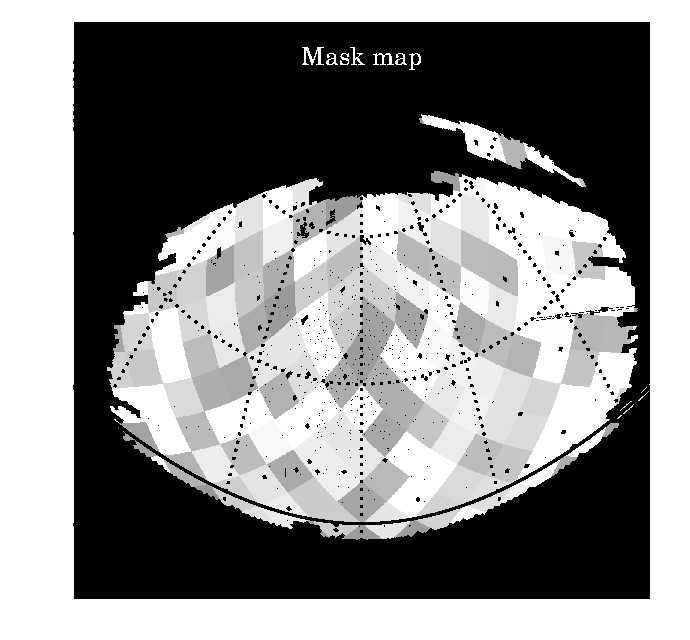
\includegraphics[width=84mm]{./plots/mask_map_plot.pdf}
\caption{The Mega-Z DR7 mask in Healpix of $N_{side}$=512. It is obtained in two steps. First, using a low resolution Healpix map of $N_{side}=64$, we reject all those pixels with less than 65 galaxies per pixel to get rid of the underpopulated areas (black patches) and obtain the overall geometry of the Mega-Z footprint. Second, we repeat the process with a star map to reject poor data quality regions of even smaller size (black dots and the long thin horizontal stripe on the right side). Different gray levels display the 174 jackknife zones used in~(\ref{covariance}) to compute the covariance of the angular correlations between different scales. They are low resolution pixels of a Healpix map with $N_{side} = 8$.}
\label{mask_map}
\end{figure}

Once we have the mask, we create the galaxy maps shown at the top of Fig.~\ref{gal_map} and the \textit{odds} maps shown at the top of Fig.~\ref{od_map}. The galaxy maps are created by counting the number of galaxies that fall in each pixel of the mask, while the \textit{odds} maps are created by averaging the \textit{odds} of these galaxies in the pixel. When no galaxies fall in a pixel, we still need an \textit{odds} value in that pixel, so we take the average value in the neighboring pixels within a circle of 1$^\circ$ radius. At the working resolution, this is a total of 19 pixels, enough so that at least one contains some galaxies, even in the last bin $0.6<z<0.65$, where the average number of galaxies per pixel is $\sim 0.36$ when the 65\% completeness cut is applied. We also create galaxy maps after applying each photo-z quality cut defined in Fig.~\ref{sigvseff}. On the second row of plots in Fig.~\ref{gal_map} we show the galaxy maps after applying the most efficient cut with 65\% completeness. 

The first \textit{odds} map at $0.45<z<0.5$ is clearly redder than the other three, since it contains galaxies with higher photo-z quality. On the contrary, bluer regions mark regions with bad photo-z quality. Note that they are not uniformly distributed on the map. They form a pattern of horizontal strips that cross the entire Mega-Z footprint. This is most noticeable in the bins $0.45<z<0.5$ and $0.5<z<0.55$. Therefore, when we remove low-\textit{odds} galaxies, we are not taking them uniformly off the map. We can already see this in the galaxy maps of Fig.~\ref{gal_map} when the {\it odds} cut is applied. If we focus on the bin $0.5<z<0.55$, we see that the map shows a strip pattern very similar to the bluer zones of its corresponding {\it odds} map. In Fig.~4 of \citet{Crocce2011} the authors show a map of the mean error on the r magnitude per pixel of a catalog similar to Mega-Z. Besides the regions with clearly bad photometry due to galactic extinction, regions with low photometric quality in the center of the footprint form patterns very similar to those on our \textit{odds} maps, with horizontal strips crossing the whole Mega-Z footprint. They approximately coincide with the drift scan paths of the SDSS instrument, and, due to observations done at different nights with different photometric quality of the atmosphere, they have resulted in regions of poor photo-z quality on the sky.
\begin{figure*}
\centering
\makebox[0cm]{\begin{tabular}{rl}
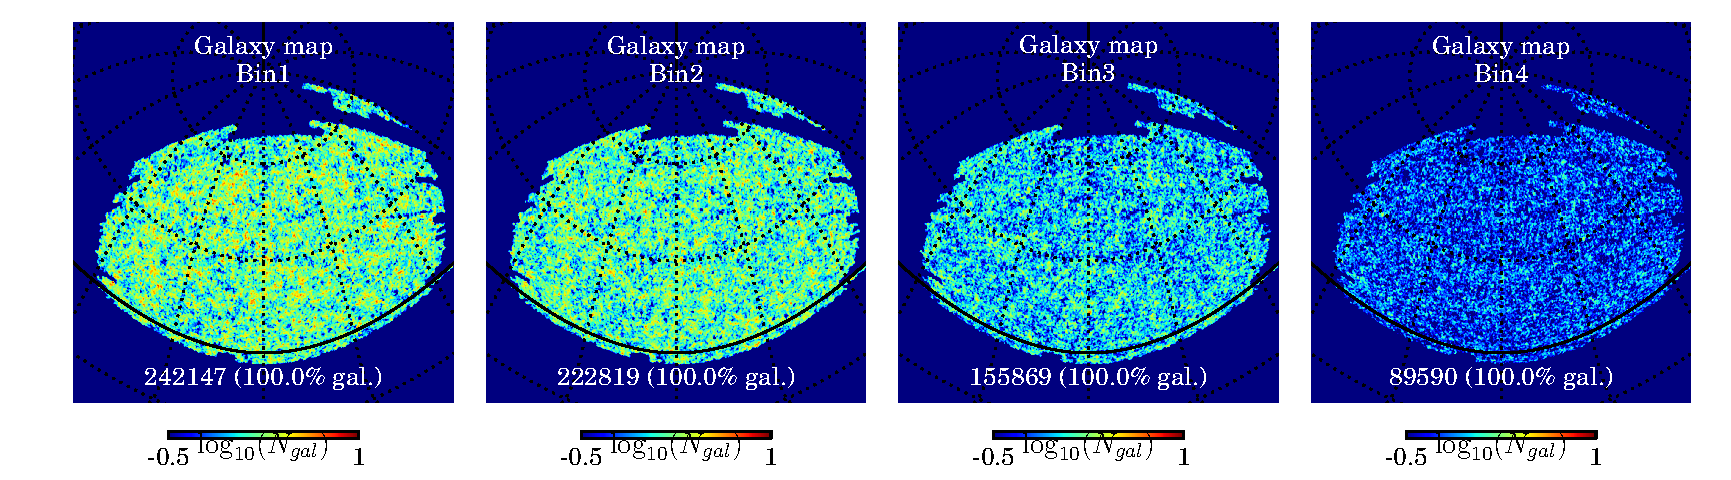
\includegraphics[width=170mm]{./plots/gal_map_plot_od100.pdf} \\
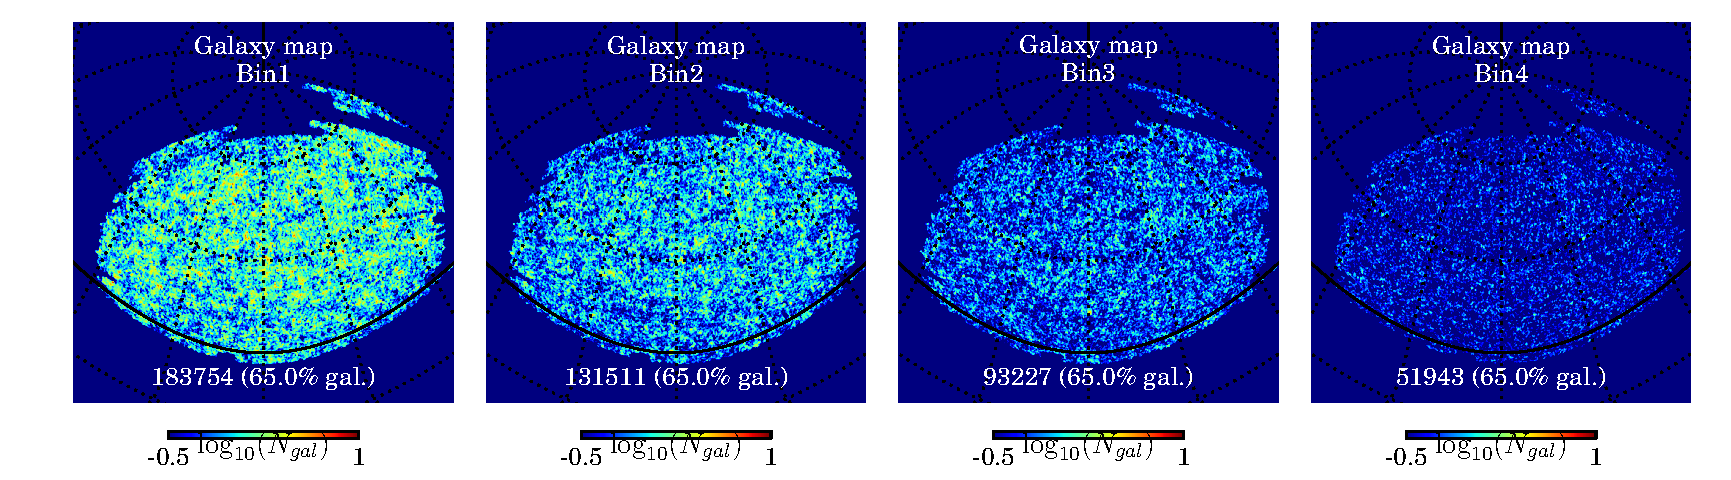
\includegraphics[width=170mm]{./plots/gal_map_plot_od65.pdf} \\
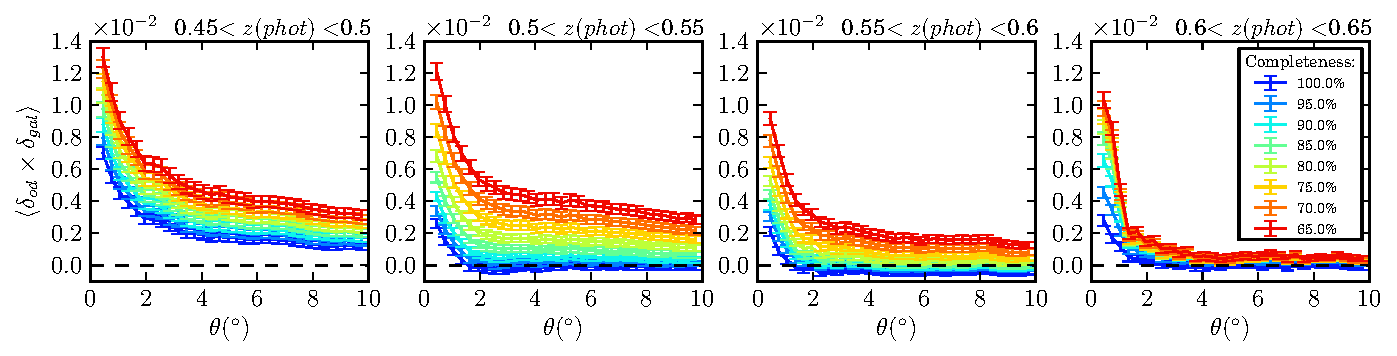
\includegraphics[width=170mm]{./plots/od_gal_corr_plot.pdf}
\end{tabular}}
\caption{On the first row, the galaxy maps of the Mega-Z catalog for the four photo-z bins of Fig.~\ref{Nz_bins}. On the second row, the same after applying a photo-z quality cut with 65\% completeness. These are Healpix maps of $N_{side}=256$. The number of galaxies is given in each map. 
On the bottom row, the angular cross correlations of the galaxy maps with the \textit{odds} maps of Fig.~\ref{od_map}, at the different photo-z quality cuts of Fig.~\ref{sigvseff}. Initially, both maps are not cross-correlated at scales $>2^\circ$ (except in the first bin, $0.45<z(phot)<0.5$), but the {\it odds} cut introduce progressively larger cross-correlations between them.}
\label{gal_map}
\end{figure*}
\begin{figure*}
\centering
\makebox[0cm]{\begin{tabular}{c}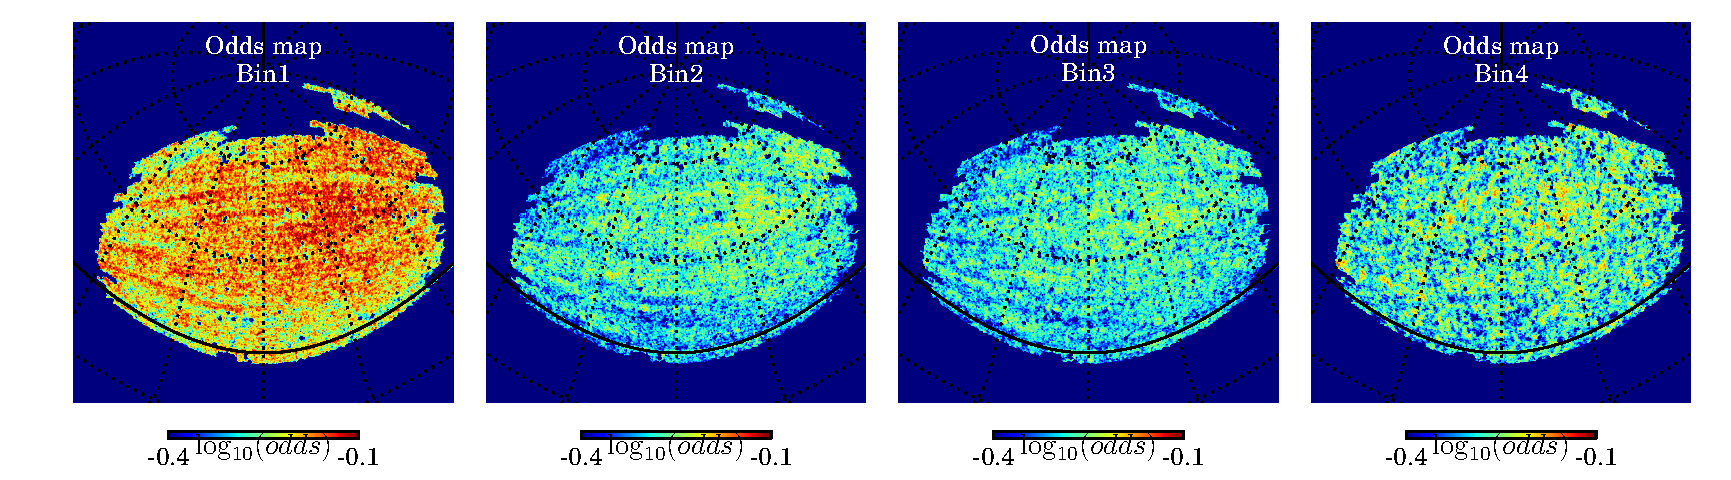
\includegraphics[width=170mm]{./plots/od_map_plot.pdf} \\
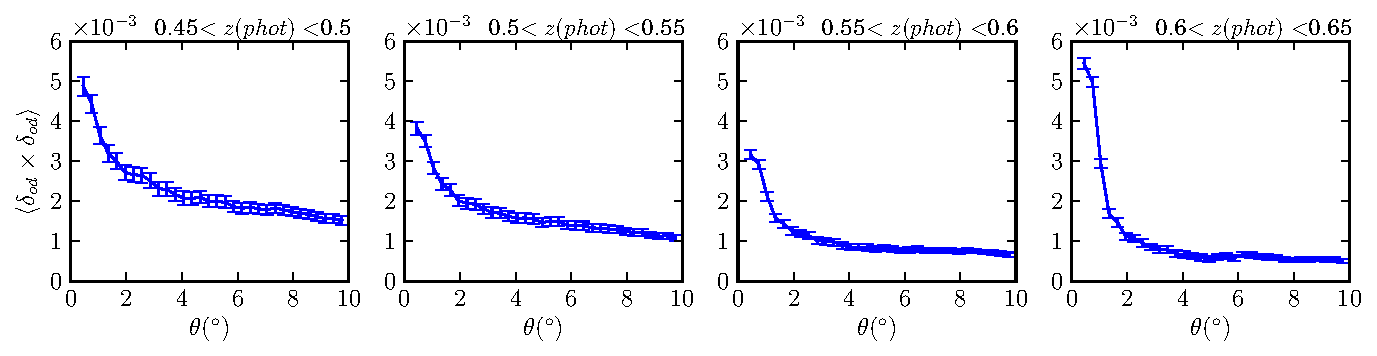
\includegraphics[width=170mm]{./plots/od_corr_plot.pdf}
\end{tabular}}
\caption{On the first row, the \textit{odds} maps of the Mega-Z catalog for the four photo-z bins of Fig.~\ref{Nz_bins}. These are Healpix maps of $N_{side}=256$ where the \textit{odds} values per pixel are computed as the mean \textit{odds} of all the galaxies in each pixel. Redder regions are regions with higher photo-z quality. They are not homogeneously distributed over the mask. 
On the bottom row, the angular auto correlations of the \textit{odds} maps. They are auto correlated at all scales $<10^\circ$, however the strength of these correlations is lower at higher $z(phot)$.}
\label{od_map}
\end{figure*}

Next we want to compute the angular correlations on all these maps. The angular correlations between two Healpix maps, $a$ and $b$, are given by:
\begin{equation}
\omega_{ab}(\theta) \equiv \langle \delta_a \delta_b \rangle (\theta) = {1 \over N_{\theta}} \sum^{N_{\theta}}_{i,j} \delta_{a,i} \delta_{b,j} \, ,
\label{measured_correlations}
\end{equation}
where $\delta_{a,i} = a_i/\bar{a} - 1$ is the fluctuation of the map $a$ at the pixel $i$ with respect to the mean $\bar{a}$, and $N_{\theta}$ is the total number of combinations of pixels $i$ and $j$ separated by an angular distance between $\theta$ and $\theta+\Delta \theta$. Since the typical pixel resolution  when $N_{side}=256$ is $\sim 0.2^\circ$, we choose $\Delta \theta$ to be $0.3^\circ$. We also want to know the covariance of $\omega_{ab}(\theta)$. We can compute it using the \textit{jackknife} technique, also used in a similar study in~\citet{Crocce2011} and explained in detail in~\citet{Cabre2007}. This technique consists of spliting the survey area within the mask into $N_k$ sub-areas. We have used pixels of a low resolution Healpix map of $N_{side}=8$ as the different jackknife sub-areas. We end up with a total of 174 pixels lying on the mask, represented by different gray levels in Fig.~\ref{mask_map}. The correlations will be computed $N_k$ times, each time removing each one of the sub-areas. This will result in the jackknife correlations $\omega_k(\theta)$. Then, the covariance between the correlation functions measured at angles $\theta_n$ and $\theta_m$ will be:
\begin{equation}
\text{Cov}_\omega(\theta_n, \theta_m) = {(N_k-1) \over (N_k)} \sum^{N_k}_{k=1}\left[ \omega_k(\theta_n) - \bar{\omega}(\theta_n) \right]\left[ \omega_k(\theta_m) - \bar{\omega}(\theta_m) \right] \, ,
\label{covariance}
\end{equation}
where $\bar{\omega}(\theta) = \sum_k^{N_k} \omega_k(\theta) / N_k$ is the mean of all the jackknife correlations. Therefore, the diagonal errors of the measured correlation at $\theta$ will be $\sigma_\omega (\theta) = \sqrt{\text{Cov}_\omega(\theta, \theta)}$.

On the bottom row of Fig.~\ref{od_map} we show the resulting auto-correlations of the \textit{odds} maps. They are not zero at any scale, which confirms that the photo-z quality is not uniformly distributed on the sky. The higher the redshift, the lower the auto correlation. However, the highest auto correlation is reached at scales $<1^\circ$ in the fourth bin, $0.6<z<0.65$. 

On the bottom row of Fig.~\ref{gal_map}, we show the resulting galaxy-\textit{odds} cross-cor\-relat\-ions, the cross-correlations between the maps on the top of this figure and those on Fig.~\ref{od_map}. Different curves of different colors label correlations after the different photo-z quality cuts in Fig.~\ref{sigvseff}. The redder curve corresponds to the most efficient cut with 65\% completeness. Apart from the first bin $0.45<z<0.5$, the general tendency is that, initially, there is little correlation between the \textit{odds} and the galaxies at scales $>2^\circ$, but once the quality cuts are applied, the cross correlations start growing. The harder the cut, the higher the correlations. However, this growth is less noticiable at higher $z$. The reason is that  the spatial features of the \textit{odds} maps become imprinted into the galaxy maps as the \textit{odds} cuts are applied. So, if the auto correlations of the \textit{odds} maps are small, the strength of this imprinting will also be small. This agrees with the behaviour of the \textit{odds} auto-correlations in Fig.~\ref{od_map}. The lower $z$ bin is unusual in the sense that the galaxy-\textit{odds} correlations are not initally 0 at any scale. This means that regions with an under- or over-density of galaxies concide with regions with the best or worst photo-z quality. This will be discussed in more detail in the following sections. Even so, the correlations still grow when the cuts are applied.

Finally, we compute the angular galaxy auto- and cross-correlation between the four photo-z bins at different photo-z quality cuts. We also compare our measured correlations with predictions. We compute the predictions for the angular correlation $\omega_{ab}(\theta)$ as described in~\cite{Crocce2011}:
\begin{equation}
\omega_{ab}^{(theo)} (\theta) = \int dz_1 N_a(z_1) \int dz_2 N_b(z_2) \xi^s(z_1,z_2,\theta) \, ,
\label{corr_prediction}
\end{equation}
where $N_i(z)$ are the selection functions, which in our case are the curves in Fig.~\ref{Nz_bins}, $\xi^s(z_1,z_2,\theta)$ is the redshift space correlation of the pairs of galaxies at redshift $z_1$ and $z_2$ subtending an angle $\theta$ with the observer. We use the non-linear power spectrum~\citep{Smith2003} with $\Lambda$CDM with $\Omega_M$ = 0.25, $\Omega_\Lambda$ = 0.75 and $H_0$ = 70~(km/s)/Mpc, the linear \citet{Kaiser1984} model of redshift space distortions for the correlation function, and a linear bias model with evolution: $b(z) = 1.5 + 0.6(z-0.1)$ \citep{Cabre2009}. We have not included the effect of magnification due to gravitational lensing, which turns out to be negligibly small for this sample. Note that the inclusion of photo-z errors in the predictions is only through the $N_i(z)$. 

The results for the auto-correlations are on the top row of Fig.~\ref{auto_odcorr}, and those for the cross-correlations are on the top row of Fig.~\ref{cross_odcorr}. Solid lines represent the predicted correlations obtained with (\ref{corr_prediction}) and points with error bars the measurements using (\ref{measured_correlations}) and (\ref{covariance}), respectively. Different colors label different photo-z quality cuts.
\begin{figure*}
\centering
\makebox[0cm]{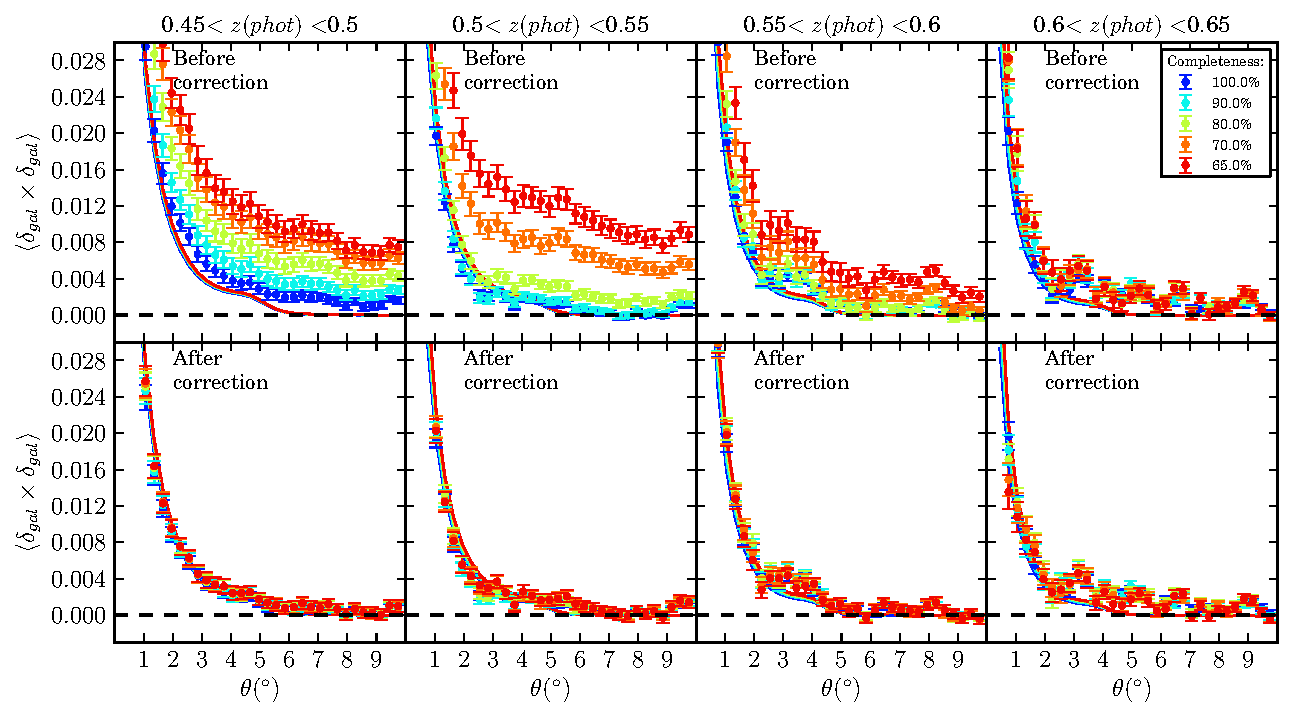
\includegraphics[width=170mm]{./plots/auto_odcorr_plot.pdf}}
\caption{The angular galaxy auto correlations in the four photo-z bins of Fig.~\ref{Nz_bins} with different photo-z quality cuts labeled with colors. The upper plots show the results before applying the \textit{odds} correction in (\ref{od_correction}), while the lower plots show the results after applying it. Points with error bars correspond to measurements and curves to predictions obtained using the $N_i(z)$ selection functions in Fig.~\ref{Nz_bins} in 
Eq.~(\ref{corr_prediction}).}
\label{auto_odcorr}
\end{figure*}

Focusing on the auto-correlations, we see that the results before any cut (blue), are slightly above the predicted curves (roughly 1 or $2\sigma$) in the first three photo-z bins, depending on the angle, and up to $\sim3\sigma$ in the last bin. The extra clustering in bin 0.6$<$z(phot)$<$0.65 is an issue already known from other studies such as \citet{Thomas2011a, Blake2008}, and, in \citet{Crocce2011}, it is justified by the fact that the number of galaxies in this bin is low enough for systematics to introduce significant distortions on the correlations. The photo-z quality cuts also introduce extra clustering, which is larger the harder the cut, as was seen in the galaxy-\textit{odds} correlations in Fig.~\ref{gal_map}. Moreover, we see that it is also related to how much the \textit{odds} are auto-correlated, since the increase of the correlations with the cut is lower at higher photo-z bins, which have smaller \textit{odds} auto-correlations (Fig.~\ref{od_map}). However, the correlations in the first bin do not increase as much as in the second bin, even having the most auto-correlated \textit{odds} map. This might be related to the fact that galaxies in this bin are already correlated with the {\it odds} value before any cut, as we can see in the bottom-left plot of Fig.~\ref{gal_map}, and, in those cases, the extra clustering may not be as additive as for a completely uncorrelated clustering.

The cross-correlations show a similar behaviour, with the photo-z quality cuts introducing extra clustering. This effect is less significant in the cross-correlation of bins 1-4, 2-4 and 3-4 than in those of bins 1-3, 2-3 and 1-2. The reason is that the fourth bin is the one whose {\it odds} map has the lowest auto correlation.
\begin{figure*}
\centering
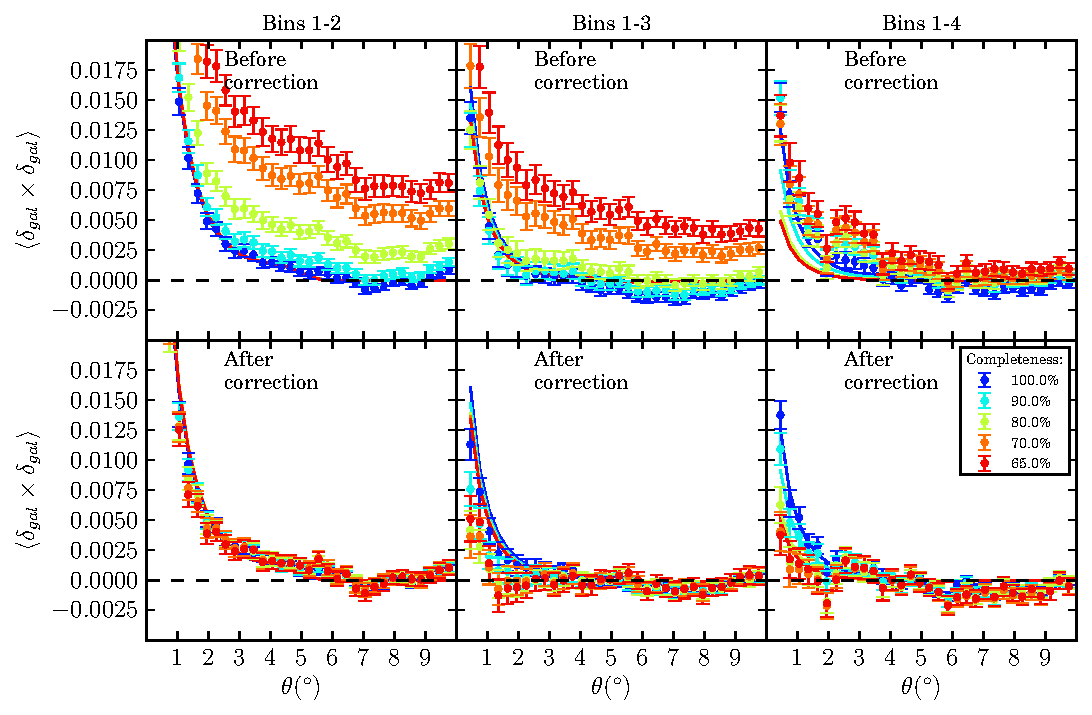
\includegraphics[width=140mm]{./plots/cross_odcorr_plot_1.pdf} \\
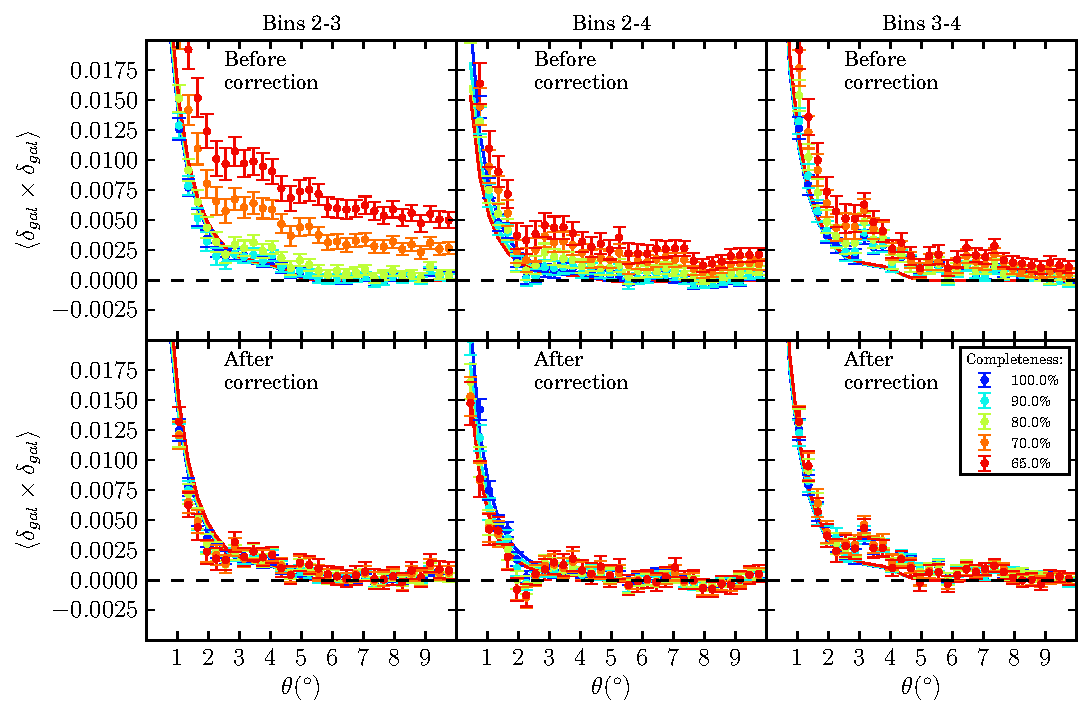
\includegraphics[width=140mm]{./plots/cross_odcorr_plot_2.pdf}
\caption{All the possible combinations of the angular galaxy cross correlations between the different photo-z bins of Fig.~\ref{Nz_bins} with different photo-z quality cuts labeled with different colors. The upper plots show the results before applying the \textit{odds} correction in~(\ref{12od_correction}), while the lower plots show the results after applying it. Points with error bars correspond to measurements and curves to predictions obtained using the $N(z)$ selections functions in Fig.~\ref{Nz_bins} in Eq.~(\ref{corr_prediction}).}
\label{cross_odcorr}
\end{figure*}
